\title[Systems Engineering]{ System Science} 

\newpage
\begin{frame}
\frametitle{ System Science }
\begin{block}{Diagram, Diagram, Diagram}

Systems engineering of now, is a science of writing instructions for people, and drawing diagrams (rather than writing code), because generally, unprepared people are easier at understanding graphics, not text.

\url{https://lockywolf.wordpress.com/2019/02/16/a-mathematical-theory-of-systems-engineering-the-elements-by-a-wayne-wymore/}

\end{block}
\end{frame}



\begin{frame}
\frametitle{ History of systems science }
\begin{figure}
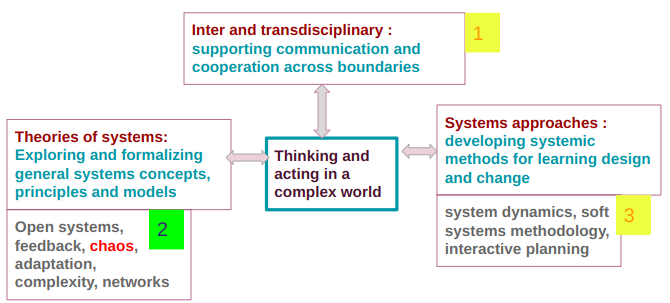
\includegraphics[scale=0.46]{pic/sysview.png}
\caption{  Three  in One }
\label{Layer1a}
\end{figure}
\end{frame}


\newpage
\begin{frame}
\frametitle{ System Science }
\begin{block}{Diagram, Diagram, Diagram}

 \url{https://onlinelibrary.wiley.com/doi/full/10.1002/sres.2215}


\end{block}
\end{frame}



\newpage
\begin{frame}
\frametitle{ System Science }
\begin{block}{Diagram, Diagram, Diagram}

\url{https://sebokwiki.org/wiki/Systems_Engineering_STEM_Overview}
\url{https://youtu.be/LjNSuL1XyV4}

\end{block}
\end{frame}


\newpage
\begin{frame}
\frametitle{ System Science }
\begin{block}{Diagram, Diagram, Diagram}

\begin{enumerate}
    \item SDS: systems dynamic society 
  \item  INCOSE : international council for system engineering   
    \item ISSS : international society for system science
    \item  computability ,  turing Machine 
\end{enumerate}

\end{block}
\end{frame}


\newpage
\begin{frame}
\frametitle{ System Science }
\begin{block}{Diagram  to Computability }

“(Alan) Turing’s work is very important; there is no question about that. He illuminated many fundamental questions. In a sense, however, it is unfortunate that he chose to write in terms of ‘computability’ especially in view of development, subsequent to Turing’s work, of modern computers. As a theory of ‘computability’, Turing’s work is quite important, as a theory of ‘computations’, it is worthless.
\end{block}
\end{frame}



\newpage
\begin{frame}
\frametitle{ System Science }
\begin{block}{Diagram  to Computability  to system dynamics }

  \begin{enumerate}
      \item physics
       \item  state variable
     \item  statistical model
      \item  relational model ( MBSE)
     \item system value models 
  \end{enumerate}
\end{block}
\end{frame}


\newpage
\begin{frame}
\frametitle{ System Science }
\begin{block}{Diagram  to Computability  to system dynamics }

 goal is to use model, not build model 
 
\end{block}
\end{frame} 

\newpage
\begin{frame}
\frametitle{ category theory }
\begin{block}{Diagram  to Computability  to system dynamics }

Formal system,
MBSE, 
requirement  relationships 

graphs 
\end{block}
\end{frame} 



\newpage
\begin{frame}
\frametitle{ more random is not good for science }
\begin{block}{.}
 \begin{figure}[scale =0.56]
\begin{tikzpicture}
		
		\begin{axis}
			[
			axis lines = left,
                ymin=0, ymax=200,
			xlabel = \( \textrm{ Complexity Variable k (int)}   \),
			ylabel = {\(   \textrm{P(X=k) Randomness} \)},
			]
		
			\addplot[  
			domain = 0:5,
			samples =10,
			color=blue]{20 + exp(x)};
		\end{axis}
	
	\end{tikzpicture}
	\caption{Complexity vs Randomness  }
	\label{poisson1d}
 
\end{figure}
 
\end{block}
\end{frame} 

